\documentclass[letterpaper, 12pt]{article}

\usepackage{caption}
\usepackage[T1]{fontenc}
\usepackage[lmargin=1 in, rmargin=1 in, tmargin=1 in, bmargin=1 in]{geometry}
\usepackage{graphicx}
\usepackage{hyperref}
\usepackage{times}
\usepackage{xcolor}

\begin{document}

\setcounter{page}{1}

\begin{center}

\textbf{Data analysis of recordings of slow earthquakes: Tectonic tremor, low-frequency earthquakes and slow slip events}

\vspace{1em}

Ariane Ducellier

PhD Dissertation Proposal

October 2019?

\end{center}

\section{Introduction}

The largest earthquakes on Earth occur in subduction zones, where large segments of the boundary between the subducting tectonic plate and the overlying plate can store energy for centuries and then release it in minutes during an earthquake. To better assess the seismic hazard, it is thus necessary to improve our understanding of subduction zone processes. Slow earthquakes are a new feature discovered in the last two decades in many subduction zones thanks to the deployment of continuously recording global positioning system (GPS) networks, and high-sensitivity borehole seismometer arrays. They can last from a few days to several years, and have a relatively short recurrence time (months to years), compared to the recurrence time of regular earthquakes (up to several hundreds of years), allowing scientists to observe and study many complete event cycles, which is typically not possible to explore with traditional earthquake catalogs. \\

Moreover, whereas regular earthquakes occur updip of the plate boundary (in the seismogenic / locked zone), slow earthquakes often occur downdip of the plate boundary, in a section adjacent to the locked section of the subduction zone. Interactions between the slow earthquakes zone and the seismogenic zone could potentially trigger large earthquakes. This phenomenon complicates our understanding of subduction zone processes, and should be taken into account when studying the seismic hazard. \\

As ordinary earthquakes, slow slip events are caused by slip on a fault such as the plate boundary between a tectonic plate subducting under another tectonic plate. However, they take a much longer time (several days to several years) to happen relative to ordinary earthquakes, and the seismic waves they generate are much weaker than the seismic waves generated by ordinary earthquakes, and may not be detectable. A slow slip event on the plate boundary is inferred to happen when there is a reversal of the direction of motion at GPS stations, compared to the secular motion of the surface displacement. Slow slip events have been observed in many subduction zones, such as Cascadia, Nankai (southwest Japan), Alaska, Costa Rica, Mexico, and New Zealand (Beroza and Ide, 2011 ~\cite{BER_2011}; Audet and Kim, 2016 ~\cite{AUD_2016}). \\

In many places, tectonic tremor are also observed in relation to slow slip. Tremor is a long (several seconds to many minutes), low amplitude seismic signal, with emergent onsets, and an absence of clear impulsive phases. Tectonic tremor have been explained as a swarm of small, low-frequency earthquakes (LFEs ; Shelly \textit{et al.}, 2007 ~\cite{SHE_2007_nature}), that is small magnitude earthquakes (M $\sim$ 1) which frequency content (1-10 Hz) is lower than for ordinary earthquakes (up to 20 Hz). The source of the LFEs is located on the plate boundary, and their focal mechanisms represent shear slip on a low-angle thrust fault dipping in the same direction as the plate interface (Ide \textit{et al.} ~\cite{IDE_2007_GRL}). Due to the lack of clear impulsive phases in the tremor signal, it is difficult to determine the depth of the tremor source with the same precision, and it is assumed to be also located close to the plate boundary. \\

LFEs are usually grouped into families of events, with all the earthquakes of a given family originating from the same small patch on the plate interface, and recurring more or less episodically in a bursty manner. The recurrence behavior of LFE families varies a lot between seismic regions, and inside the same seismic region. In Washington State, LFE swarm duration, recurrence interval, and event size decrease systematically with increasing depth (Sweet \textit{et al.}, 2019 ~\cite{SWE_2019}). On the San Andreas Fault, the recurrence behaviors of LFE families vary from highly episodic (large episodes every few months) to semicontinuous (small episodes every few days), and some LFE families exhibit variability in recurrence behavior over time, from semicontinuous to episodic (Shelly, 2017 ~\cite{SHE_2017}). \\

In subduction zones such as Nankai and Cascadia, tectonic tremor observations are spatially and temporally correlated with slow slip observations (Obara, 2002 ~\cite{OBA_2002}; Rogers and Dragert, 2003 ~\cite{ROG_2003}). Due to this correlation, these paired phenomena have been called Episodic Tremor and Slip (ETS). However, in Cascadia only the biggest tremor episodes are associated with slow slip events. Smaller slow slip events may occur at the same time as the smaller bursts of tremor, but if they exist, they are currently undetected. Moreover, in northern New Zealand, tremor and slow slip do not seem to be spatially and temporally correlated. Tremor is more challenging to detect, seems to be located downdip of the slow slip on the plate boundary, and the tremor activity does not seem to increase during slow slip events.

\section{Proposed PhD Research}

The purpose of my research is to carry out data analyses of recordings of tectonic tremor, low-frequency earthquakes and slow slip events to better understand the mechanism of slow earthquakes. Specifically, I intend to answer the following questions:

\begin{itemize}
\item Is the source of the tectonic tremor located on the plate boundary? What is the depth extent of the location of the source of the tremor?
\item Do low-frequency earthquakes families behave similarly or differently in Northern California, compared to Washington State and the San Andreas Fault?
\item Can we detect smaller and / or longer slow slip events in the absence of spatially and temporally correlated tectonic tremor?
\end{itemize}

My PhD thesis will be comprised of five chapters. The first chapter will be an introduction and literature review of slow earthquake phenomena. The second, third, and fourth chapters will be journal articles detailing the methods used to answer the previous questions, and what it can tell us on the causes and mechanisms of slow earthquakes. The final chapter will synthesize my research into conclusions and potential future avenues of research.

\subsection{Depth of the source of the tectonic tremor in the eastern Olympic Peninsula}

\textit{Is the source of the tectonic tremor located on the plate boundary? What is the depth extent of the location of the source of the tremor?}

\subsubsection{Introduction}

Tremor is a long (several seconds to many minutes), low amplitude seismic signal, with emergent onsets, and an absence of clear impulsive phases. Tectonic tremor have been explained as a swarm of small, low frequency earthquakes ~\cite{SHE_2007}, that is small magnitude earthquakes (M $\sim$ 1) which frequency content (1-10 Hz) is lower than for ordinary earthquakes (up to 20 Hz). The source of the low-frequency earthquakes is located on the plate boundary, and their focal mechanisms represent shear slip on a low-angle thrust fault dipping in the same direction as the plate interface ~\cite{IDE_2007}. Due to the lack of clear impulsive phases in the tremor signal, it is difficult to determine the depth of the tremor source with the same precision, and it is assumed to be also located close to the plate boundary. In subduction zones such as Nankai and Cascadia, tectonic tremor observations are spatially and temporally correlated with slow slip observations ~\cite{OBA_2002}; ~\cite{ROG_2003}. Due to this correlation, these paired phenomena have been called Episodic Tremor and Slip (ETS).

\subsubsection{Data}

The data were collected during the 2009-2010 Array of Arrays experiment. Eight small-aperture arrays were installed in the northeastern part of the Olympic Peninsula, Washington. The aperture of the arrays was about 1 km, and station spacing was a few hundred meters. The arrays were around 5 to 10 km apart from each other (Figure 1). Most of the arrays were installed for more than a year, between June 2009 to September 2010, and were able to record the main August 2010 ETS event. Some of the arrays were also recording during the August 2011 ETS event. ~\cite{GHO_2012} used a multibeam-backprojection (MBBP) technique to detect and locate tremor. They bandpass filtered the seismic data between 5 and 9 Hz. They divided the data into one-minute-long sliding independent (no overlap) time windows. They performed beam forming in the frequency domain at each array to determine the slowness vectors, and backprojected the slownesses in the 3-D space to locate the source of the tremor for each time window. We thus have two catalogs of tremors. The first one is a catalog of 28902 one-minute-long time windows during which tremor was detected between June 20th 2009 and September 30th 2010. For each time window, we have the beginning time, the end time, and the location (latitude and longitude) of the source of the tremor. The second one is a catalog of 5600 one-minute-long time windows between August 10th 2011 and September 6th 2011.

\subsubsection{Method}

We took a 5 km by 5 km grid cell located not too far (less than 25 km) from a given array. We then took all the one-minute-long time windows when tremor was detected and the source of the tremor was located inside this cell. For each one-minute-long time window, we downloaded the seismic data for each seismic station of the array. Then, for each seismic station and each channel, we detrended the data, tapered the first and last 5 seconds of the data with a Hann window, removed the instrument response, bandpass filtered between 2 and 8 Hz, and resampled the data to 20 Hz. All these preprocessing operations were done with the Python package obspy. For each seismic station and each one-minute-long time window, we cross correlated the vertical component with the East-West horizontal component and the North-South horizontal component. Then, we stacked the cross correlation functions over all the seismic stations of the array. We experimented with a linear stack, a power stack, and a phase-weighted stack. Figure 2 shows an example of the cross correlation functions as function of time for the Big Skidder array for the 82 one-minute long time windows when tremor was detected in a 5 km by 5 km grid cell centered on the array. We can see that for about half of the tremor windows, there is a peak in the cross correlation at about 4.7 s. As the energy of the P-waves is expected to be higher on the vertical component, and the energy of the S-waves to be higher on the horizontal components, we assume that this peak corresponds to the time lag between the arrival a direct P-wave and a direct S-wave. We then stacked the cross correlation functions over all the one-minute-long time windows. Again, we experimented with a linear stack, a power stack, and a phase-weighted stack. We assume that the time of the maximum absolute value of the peak of the stack is the time lag between the arrival of the direct P-wave and the arrival of the direct S-wave. \\

Only about half of the cross correlation functions have a distinct peak that coincides with the peak in the stacked cross correlation. The other cross correlations functions show either a distinct peak at another time lag, or no clearly visible peak. This may be due either because the source of the tremor during the corresponding one-minute-long time window was mislocated, either because the signal-to-noise ratio is too low. To improve the signal-to-noise ratio of the peak in the stacked cross correlation, we divided the one-minute-long time windows into two clusters, the ones that match well the stacked cross correlation, and the ones that do not math it well. For each one-minute-long time window, we compute the maximum absolute value of the cross correlation, its value at time 0, the time at which we takes its maximum absolute value, and the ratio between the
amplitude of the cross correlation peak to the root mean square error of the cross correlation function. We do this for both the East-West component and the North-South component, Each one-minute-long time window is thus associated to eight values of quality criteria. We then classified each one-minute-long time window into two different clusters, based on the value of these criteria, using a k-means clustering algorithm (function sklearn.cluster.KMeans from the Python library SciKitLearn). For each cluster, we then stacked the cross correlation functions over all the one-minute-long time windows belonging to the cluster. Figure 3 shows the stacked cross correlation for each of the clusters compared to the original stacked cross correlation for all the one-minute-long time windows. The clustering has improved the amplitude of the peak for one of the clusters, and made the peak nearly disappear for the other cluster. \\

We did this analysis for grid cells located in a 50 km by 50 km area centered on each of the eight arrays. We thus have 121 * 8 = 968 values of the time lag between the arrival of the direct P-wave and the arrival of the direct S-wave. We first assumed that the source of the tremor is located on the plate boundary, and we took a 1D velocity model for the overriding continental crust with $V_P$ = 6.4 km/s and $V_S$ = 3.6 km/s, to compute the depth of the tremor source for each location. \textcolor{red}{Modify this part if we use a 3D velocity model.}

\subsubsection{Results}

The analysis we carried out above may not lead to a reliable value of the depth of the source of the tremor for all relative positions of the array and the tremor. First, some areas are badly covered, and only a few tremor or no tremor at all were recorded. We limit our analysis to grid cells were tremor has been recorded during at least \textcolor{red}{10 (to be modified?)} one-minute-longtime windows. Another problem is that we assumed that the location of the tremor source is fixed during the one-minute-long time window where we compute the cross correlation of the seismic signal. However, this is not exactly the case. Indeed, during an ETS event, rapid tremor streaks have been observed propagating in the up-dip and down-dip directions at velocities ranging on average between 30 and 110, and up to 200 km/h \cite{GHO_2010_G3}, which corresponds to a source displacement of 0.5, 1.8, and 3.3 km during one minute. If we denote $t_P$ the arrival time of the direct P-wave, and $t_S$ the arrival time of the direct S-wave, the time lag between the two phase arrivals is $t_{lag} = t_S - t_P$. During the one-minute time window where we compute the cross correlation, the displacement $dx$ of the tremor source along the plate boundary should corresponds to a time lag difference $dt_{lag}$ shorter than a quarter of the dominant period of the tremor signal $T$ = 0.3 s. We computed the time lag difference for a displacement of the source of 0.5, 1.8 and 3.3 km in the up-dip direction, for stations aligned along the strike and along the dip direction. We assume that the source was located at 35 km depth, and we look at the time arrivals of the seismic wave for stations located up to 20 km from the epicenter, in the strike or the dip direction. The difference in time lags stays low for all the stations aligned along the strike of the plate boundary, even for tremor streaks traveling at 200 km/h. However, for the stations aligned along the dip of the plate boundary, the tremor streaks traveling at 200 km/h will cause a problem for the stations that are not immediately above the tremor source. The tremor streaks traveling at 110 km/h will cause a problem for the stations located more than 6 km updip of the tremor source. \\

\textcolor{red}{Something about how we choose the values we are keeping.} \\

\textcolor{red}{Something about interpolating the values of the different arrays.} \\

\textcolor{red}{Include here Figure 4 of the distance to the plate boundary + include values for the LFE families.} \\

\subsubsection{Discussion}

In the above part, we assumed that all the tremor within a given grid cell originate from the same depth, and we averaged over all the data to get the depth of the tremor source. However, instead of being located on the same plane near the plate boundary, the tremor may be scattered over a layer surrounding the plate boundary. To compute the thickness of this layer, we compute for each one-minute-long time window for which the cross correlation function matches well the stacked cross correlation the time lag between the time corresponding to the maximum absolute value for the cross correlation function and the time corresponding to the maximum absolute value for the stacked cross correlation. We then compute the standard deviation of this time lag, and compute the corresponding difference in depth using the 1D velocity model that we used previously.   \textcolor{red}{Something about computation of robust standard deviation.} We thus get the thickness of the layer from which the tremor originate. We used the same interpolation method as above to get the thickness of the layer for all the area covered by the eight arrays. Figure 5 shows the map of the thickness. \\

\textcolor{red}{Some interpretation.}

\subsubsection{Conclusion}

How analysis addresses the part of the specific question

How analysis addresses the specific question

How analysis addresses the general question

\subsection{A low-frequency earthquakes catalog for Northern California}

\textit{Do low-frequency earthquakes families behave similarly or differently in Northern California, compared to Washington State and the San Andreas Fault?}

\subsubsection*{Motivation}

The relatively short recurrence of slow slip and tremor events results in a rich history both in space and time and reveals potential patterns.  These event histories have allowed scientists to see complete event cycles, which is typically not possible to explore in traditional earthquake catalogs. However, most of the work on low-frequency earthquakes (LFEs) has been focused on detecting LFEs during periods of high tremor activity, grouping them into families of events, and locating the source of the LFE families. Longer catalogs (several years) have been established for LFE families in Mexico (two-year long catalog by Frank \textit{et al.}, 2014 ~\cite{FRA_2014}), the San Andreas Fault (fifteen-year-long catalog by Shelly, 2017 ~\cite{SHE_2017}), and Washington State (five-year-long catalog by Sweet \textit{et al.}, 2019 ~\cite{SWE_2019} and two-year-long catalog by Chestler and Creager, 2017a ~\cite{CHE_2017_JGR} and b ~\cite{CHE_2017_G3}). These studies have shown that LFEs can show a wide range of different behaviors. In northern Washington, Sweet \textit{et al.} (2019) have identified and characterized four different LFE families that span the width of the transition zone in the Cascadia Subduction Zone beneath western Washington State. They found that the LFEs swarm duration, recurrence interval, and event size decrease systematically with increasing depth. On the San Andreas Fault, Shelly (2017 ~\cite{SHE_2017}) observed a large diversity of recurrence behaviors among the LFE families, from semicontinuous to highly episodic. Particularly, two families exhibited bimodal recurrence patterns (about 3 and 6 days for the first one, and about 2 and 4 days for the second one). Moreover, he observed an increase in the LFE event rate after the 2004 Parkfield earthquake. \\

Plourde \textit{et al.} (2015 ~\cite{PLO_2015}) have detected LFEs in southern Cascadia during the April 2008 Episodic Tremor and Slip event using seismic data from the EarthScope Flexible Array Mendocino Experiment (FAME). They used a combination of autodetection methods and visual identification to obtain the initial templates. Then, they recovered higher signal-to-noise LFE signals using iterative network cross correlation. They found that the LFE families on the southern Cascadia Subduction Zone were located above the plate boundary, with a large distribution of depths (28-47 km). Three additional LFE families were found on two strike-slip faults, the Maacama and Bucknell Creek faults, which are part of the San Andreas Fault zone. \\

I intend to extend the catalog from Plourde \textit{et al.} (2015 ~\cite{PLO_2015}) to the whole two years during which the temporary seismic stations from the FAME experiment were installed, (and possibly to a longer period if the quality of the seismic data allows it) in order to answer two questions:

\paragraph{How is low-frequency earthquakes event rate affected by nearby earthquakes?} I intend to study how LFE families respond to local perturbations in stress from nearby earthquakes at the Mendocino Triple Junction. The deformation, tectonics, and evolution of southern Cascadia is strongly influenced by the Mendocino Triple Junction, and the Mendocino Triple Junction is one of the most seismically active regions along the Cascadia Subduction Zone. Tremor intensity is affected by regular earthquakes. For instance, tremor in Cascadia is triggered by stresses caused by surface waves from large, distant earthquakes (Rubinstein \textit{et al.}, 2009 ~\cite{RUB_2009}), tremor on the San Andreas Fault is triggered by regional earthquakes (Peng \textit{et al.}, 2009 ~\cite{PEN_2009}; Guilhem \textit{et al.}, 2010 ~\cite{GUI_2010}), and small intraslab earthquakes in Nankai, Japan have also been found to trigger tremor (Han \textit{et al.}, 2014 ~\cite{HAN_2014}). I intend to verify whether a similar pattern can be observed for LFEs. 

\paragraph{Are there differences or similarities with the San Andreas Fault, and northern Cascadia?} I intend to study how the behavior of the LFE families identified by Plourde \textit{et al.} (2015  ~\cite{PLO_2015}) on the two strike-slip faults is similar or differ from the behavior of the LFE families located on the southern Cascadia Subduction Zone. In particular, I would like to verify whether the LFE families located on the Maacama and Bucknell Creek fault have a similar behavior to what was observed by Shelly (2017 ~\cite{SHE_2017}) on the San Andreas Fault, and whether the LFE families located on the southern Cascadia Subduction Zone have a similar behavior to what was observed by Sweet \textit{et al.} (2019 ~\cite{SWE_2019}) on the northern Cascadia Subduction Zone. \\

Once I have obtained the new two-year-long catalog of LFEs, I intend to carry out a more thorough statistical analysis of the occurrence of LFE events. Specifically, I will study how some statistical features of LFE catalogs compare to statistical features of regular earthquake catalogs. It has been shown that whereas the frequency distribution of the magnitude of regular earthquakes follows a power law with b-value $\sim$ 1, the frequency distribution of the magnitude of LFEs follows either a power law with a higher b-value ($\sim$ 5, Bostock et al., 2015 ~\cite{BOS_2015}) or an exponential law (Sweet et al., 2014 ~\cite{SWE_2014}; Chestler and Creager, 2017a ~\cite{CHE_2017_JGR}). I would like to verify whether LFE catalogs and regular earthquake catalogs differ for other statistical features as well. I will explore two problems:

\paragraph{Long-range dependence (or self-similarity)} Long-range dependence is a phenomenon that may arise in the statistical analysis of time series data. It relates to the slow rate of decay of the statistical dependence between two points with increasing time interval between the points. Evidence of long-range dependence has been found in regional earthquakes catalogs (Telesca \textit{et al.}, 2000; Li \textit{et al.}, 2002; Telesca \textit{et al.}, 2004; Enescu \textit{et al.}, 2006; Jimenez \textit{et al.}, 2006; Xu and Burton, 2006; Bunde and Lennartz, 2012; Wang, 2013; Gkarlaoui \textit{et al.}, 2017; Telesca \textit{et al.}, 2017; Barani \textit{et al.}, 2018; Matcharashvili \textit{et al.}, 2018; Mukhopadhyay and Sengupta, 2018), global earthquakes catalogs (Ogata and Abe, 1991; Sarlis \textit{et al.}, 2018), and in catalogs of mining-induced seismicity (W\k{e}glarczyk and Lasocki, 2009). We can investigate whether there is long-range dependence in a catalog by computing the fractional index $d$, which represents how fast the variance in the number of LFEs in a time window of a given length increases with the length of the time window considered. A fractional index such that $0 < d < 0.5$ is characteristic of long-range dependence in the time series, whereas a Poisson process has a fractional index equal to 0. I intend to compute the fractional index for all the families in the new two-year-long LFE catalog for southern Cascadia, and compare it to the fractional index obtained for catalogs in Mexico (Frank \textit{et al.}, 2014 ~\cite{FRA_2014}), the San Andreas Fault (Shelly, 2017 ~\cite{SHE_2017}), and Washington State (Sweet \textit{et al.}, 2019 ~\cite{SWE_2019} and Chestler and Creager, 2017a ~\cite{CHE_2017_JGR} and b ~\cite{CHE_2017_G3}). \\

This kind of statistical analysis may help explain the mechanism producing LFEs. If slow slip was an increase of the loading rate on the plate boundary, it should increase the rate of LFEs, but their distribution should still follow a Poisson process. If the fractional index $d$ is higher than 0, it would seem to imply than the occurrence of LFEs does not follow a Poisson process, and that the density of asperities increases during a slow slip event (Frank \textit{et al.}, 2016 ~\cite{FRA_2016_SA}). A possible explanation is that a large number of asperities are locked during the inter-slip period, and are activated during slow slip by a mechanism such as migrating pore pressure pulses (Frank \textit{et al.}, 2015 ~\cite{FRA_2015}), or along-fault hydrofracturing similar to what is geologically observed on ancient subduction zones (Angiboust \textit{et al.}, 2015 ~\cite{ANG_2015}).

\paragraph{Temporal models of seismicity} Temporal models of seismicity have been developed to describe, analyze and forecast the probabilities of regular earthquake occurrences. The Epidemic-Type Aftershock Sequence (ETAS) model was first introduced by Ogata (1988 ~\cite{OGA_1988}). It takes account the magnitude frequency distribution law of Gutemberg and Richter (1944 ~\cite{GUT_1944}) and the Omori-Utsu law of aftershock decay (Omori, 1894 ~\cite{OMO_1894}; Utsu, 1957 ~\cite{UTS_1957}), but it allows each event, irrespective of whether it is a small or a big event, to trigger its own offspring. According to the Omori-Utsu formula, the number of aftershocks after a mainshock decays as $1 / t^p$, where $t$ is the time from the occurrence of the main shock, and the decay rate $p$ can vary between 0.9 and 1.5 (Utsu \textit{et al.}, 1995 ~\cite{UTS_1995}). I intend to first verify whether I can fit an ETAS model to the available LFE catalogs, and then verify whether the decay rate for LFE catalogs is similar to the decay rate obtained for regular earthquake catalogs. \\

\textcolor{red}{Add something about earthquake-rate equations from Dieterich should lead to p = 1}

\subsubsection*{Completed work}

\paragraph{Extension of the LFE catalog} Alexandre Plourde has kindly accepted to share his LFE catalog with me. For each LFE family, each seismic station, and each channel (two horizontal and one vertical), I have downloaded a one-minute-long time window of seismic data around the detection time of each LFE. I have then linearly stacked the data to obtain a template for each LFE family, each seismic station, and each channel. I then used a matched-filter algorithm. To detect new LFEs for a given LFE family, I download one hour of seismic data. Then for each station and each channel, I cross-correlate the one-hour long signal with the one-minute-long template for the given station and channel. As the signal-to-noise ratio of the seismic data is low, we may not see obvious peaks in the cross-correlation signal. However, if we stack the cross-correlation signals for all the channels and all the stations, we can see peaks appearing. Whenever the value of the average cross-correlation is higher than a threshold (generally eight times the median absolute deviation), I assume that there is a LFE. \\

I first applied the matched-filter algorithm on the time period covered by the catalog of Plourde \textit{et al.} (2015 ~\cite{PLO_2015}), and compared the LFE detection times I obtained to the detection times in the original catalog. I have successfully detected nearly all the LFE events that were present in the original catalog and added a few new LFEs (see Table X for an example for family 080421.14.048). I missed only two LFEs, but one of them was preceded by another LFE 1.95 seconds before, and the other one was followed by another LFE 3.375 seconds later. In the catalog by Plourde \textit{et al.} (2015 ~\cite{PLO_2015}), these LFEs were considered as separate LFEs, but it is possible that the peaks in the cross correlation correspond in fact to the same LFEs. I added 13 LFEs to the catalog but they all have a small cross correlation value compared to the other LFEs in the catalog, and they may be false detections. I have reproduced the detection times with similar accuracy for all the LFE families in the original catalog. \\

I have then used the matched-filter algorithm to extend the catalog to the period 2007-2009 using first both the FAME stations and the permanent stations, and then only the permanent stations (Figure X), for two different LFE families, one located on the southern Cascadia Subduction Zone (family 080421.14.048), and one located on a strike-slip fault from the San Andreas Fault system (family 080326.08.015). For the subduction zone family, I was able to detect the burst of LFEs during the April 2008 ETS event even when I used only the templates from the permanent stations. The results are more contrasted for the strike-slip fault family. I was able to detect most of the main bursts of LFEs when I used only the templates from the permanent stations, but I missed a few bursts of LFEs. This may be due because I have only two seismic stations with three components, the other five seismic stations that I used recorded only the vertical component. Due to the reduced number of channels available, I probably have more false detections. The stations from the permanent networks have been recording seismic data from at least 2007 until now, and I infer that I will be able to extend the catalog from 2009 to 2019 using only seismic data from the permanent stations.

\paragraph{Statistical analysis of LFE catalogs} I have analyzed catalogs of LFEs from Mexico (Frank \textit{et al.}, 2014 ~\cite{FRA_2014}), the San Andreas Fault (Shelly, 2017 ~\cite{SHE_2017}), and Washington State (Sweet \textit{et al.}, 2019 ~\cite{SWE_2019} and Chestler and Creager, 2017a ~\cite{CHE_2017_JGR} and b ~\cite{CHE_2017_G3}). I also analyzed the original LFE catalog of Plourde \textit{et al.} (2015 ~\cite{PLO_2015}). For each family of LFEs, I translated the catalog into a continuous time series defined by number of events per minute. The sample interval is 1 minute. Then, I computed the value of the fractional parameter $d$, which represents how fast the variance in the number of LFEs increases with the length of the time window considered. Following Taqqu and Teverovsky (1998 ~\cite{TAQ_1998}), I computed this parameter using the absolute value method, the variance method, the variance of residuals method the R/S method, and the periodogram method. These methods gave values of $d$ that are consistent between one method and another, except for the absolute value method, and the R/S method. These may be due because these methods assume that the time series is stationary, which may not be the case is the time period studied is too short and only one burst of LFEs during a big ETS event has been recorded. The results of the computation of the fractional parameter with the variance method fro the four regional areas considered are shown in Figures X to X. For most families of the catalogs studied, I found that $0 < d < 0.5$, which is characteristic of long-range dependence in the time series. The only exception is the San Andreas Fault catalog, where the LFE families show a wider range of behaviors, and where only some of the families exhibit evidence for long-range dependence.

\subsubsection*{Future work}

\paragraph{Extension of the LFE catalog} I will first use the templates to extend the LFE catalog by Plourde \textit{et al.} (2015) to the period 2007-2009 for all the LFE families in the catalog, as I have already done for two LFE families. Then for each LFE family, I will choose about one hundred LFEs with the best values of the cross correlation coefficient to compute templates for nearby (within a hundred kilometers) permanent stations that were recording during the 2007-2009 period. I will then use these new templates to find LFEs during the same period, and I will compare the catalog computed with the temporary stations from the FAME network and the catalog computed with the permanent stations. If for a given family, I can retrieve most of the LFEs detected with the temporary FAME network when I use only the permanent stations, I will then extend the LFE catalog to the period 2009-2019. \\

I will then study how low-frequency earthquakes event rate is affected by nearby earthquakes. I will take several moderate earthquakes that occurred near the Mendocino Triple Junction, and test whether there is a change in the LFE event rate before and after the earthquakes. I intend particularly to test the effects of the M5.4 April 30th 2008 earthquake, and the M6.5 January 10th 2010 earthquake. Shelly (2017 ~\cite{SHE_2017}) noticed changed in the LFE event rate for some LFE families for at least several months after the M6.0 2004 Parkfield earthquake on the San Andreas Fault. I will also compare the behavior of the most updip LFE families with the behavior of the most downdip LFE families, and verify whether the downdip families are more frequently active than the updip families, as observed by Sweet \textit{et al.} (2019 ~\cite{SWE_2019}) in Washington state.

\paragraph{Statistical analysis of LFE catalogs} Once I have obtained a two-year-long LFE catalog, I will recompute the value of the fractional parameter for all the LFE families, as I have already done for the two-month-long catalog by Plourde \textit{et al.} (2015 ~\cite{PLO_2015}), and I will verify if I still observe evidence for long-range dependence. I will then try to fit an ETAS model on the available LFE catalogs. I will start with the catalog by Chestler and Creager (2017a ~\cite{CHE_2017_JGR} and b ~\cite{CHE_2017_G3}) because it provides values for the magnitudes of the LFEs. However, it should be possible to fit an ETAS model with the other catalogs as well, by assuming that all the LFEs have the same magnitude, or by looking at the amplitude of the seismic waveforms instead of the magnitude. I intend to use the software R and two available R packages, bayesianETAS by Gordon Ross ~\cite{ROS_2016}, and PtProcess by David Harte ~\cite{HAR_2010}.

\subsection{Detection of slow slip events in New Zealand}

\textit{Can we detect smaller and / or longer slow slip events in the absence of spatially and temporally correlated tectonic tremor?}

\subsubsection*{Motivation}

As ordinary earthquakes, slow slip events are caused by slip on a fault such as the plate boundary between a tectonic plate subducting under another tectonic plate. However, they take a much longer time (several days to several years) to happen relative to ordinary earthquakes, and the seismic waves they generate are much weaker than the seismic waves generated by ordinary earthquakes, and may not be detectable.  A slow slip event on the plate boundary is inferred to happen when there is a reversal of the direction of motion at GPS stations, compared to the secular motion of the surface displacement. Slow slip events have been observed in many subduction zones, such as Cascadia, Nankai (southwest Japan), Alaska, Costa Rica, Mexico, and New Zealand (Beroza and Ide, 2011 ~\cite{BER_2011}; Audet and Kim, 2016 ~\cite{AUD_2016}). \\

In many places, tectonic tremor are also observed in relation to slow slip. In subduction zones such as Nankai and Cascadia, tectonic tremor observations are spatially and temporally correlated with slow slip observations (Obara, 2002 ~\cite{OBA_2002}; Rogers and Dragert, 2003 ~\cite{ROG_2003}). Due to this correlation, these paired phenomena have been called Episodic Tremor and Slip. However, this is not always the case. For instance, in northern New Zealand, tremor are more challenging to detect, and seem to be located downdip of the slow slip on the plate boundary. \\

New Zealand exhibits a wide range of slow slip behavior, and is therefore an exciting site for research. The tectonics of the North Island of New Zealand is dominated by the westward subduction of the Pacific Plate under the Australian Plate at the Hikurangi Trench. Two types of slow slip events have been observed at the Hikurangi margin. Shallow (10-15 km depth), shorter (1-3 weeks), and usually smaller (Mw 6.3-6.8) slow slip events have been observed every 18-24 months in the northern part of the margin. Deeper (35-60 km depth), longer (12-18 months), and larger (Mw 7.0) slow slip events have been observed every 5 years in the southern part of the margin (Wallace and Beavan, 2010 ~\cite{WAL_2010}; Todd and Schwartz, 2016 ~\cite{TOD_2016}).\\

It used to be thought that there were no tremor associated with slow slip events in northern Hikurangi. Delahaye \textit{et al.} (2009 ~\cite{DEL_2009}) observed an increase in the rate of microseismicity downdip of the 2004 Gisborne slow slip event. More recently however, Kim \textit{et al.} (2011 ~\cite{KIM_2011}) detected a low level of tremor activity that increased during the 2010 Gisborne slow slip event. As was the case for the microearthquakes, the source of the tremor was located downdip of the slow slip patch determined from GPS data. Ide (2012 ~\cite{IDE_2012}) detected tremor downdip of the location of two deep slow slip events observed by Wallace and Eberhart-Phillips (2013 ~\cite{WAL_2013}) in 2006 and 2008. However, contrary to Episodic Tremor and Slip (ETS) events in Cascadia and Nankai, the tremor activity did not seem to increase during the slow slip events. Todd and Schwartz (2016 ~\cite{TOD_2016}) detected tremor associated with most of the shallow slow slip events between 2010 and 2015, and located downdip of the geodetically inferred slip area. They also detected deeper tremor between 20 and 50 km depth with unclear origin. They hypothesized that these tremor may be related to currently undetected deep long-term slow slip events.\\

In other subduction zones, tremor has been used as a proxy to study slow slip events. For instance, Aguiar \textit{et al.} (2009 ~\cite{AGU_2009}) used the tremor occurrence rate to determine the moment released by short tremor episodes for which no slow slip is detectable in the GPS data. Frank (2016 ~\cite{FRA_2016_GRL}) stacked independently the displacement observed on GPS data during time periods when low-frequency earthquakes are detected, and the displacement observed during time periods when no low-frequency earthquake is detected, and succeeded in observing surface deformation previously hidden in GPS noise. However, as there is no clear relationship between tremor and slow slip occurrence in New Zealand, these methods cannot be applied, and we need other methods to be able to better detect and quantify slow slip.\\

Several questions could be explored regarding slow slip in northern New Zealand:

\paragraph{Detecting smaller, currently undetected slow slip events.} This would help us to verify whether the fault weakens with depth. Indeed, it has been observed in Cascadia that, with decreasing depth, there is a gradation from frequent tremor episodes with small spatial and temporal extent, to infrequent tremor episodes with large spatial and temporal extent (Wech and Creager, 2011 ~\cite{WEC_2011}). The same behavior was observed for low-frequency earthquakes (LFEs) with downdip LFEs swarms happening nearly weekly and updip families only occurring during the yearly ETS events (Sweet \textit{et al.}, 2019 ~\cite{SWE_2019}). As there is a temporal and spatial correlation between slow slip, tremor and LFEs, the same spatial pattern is also expected for the slow slip. However, the limited resolution of geodetic instruments only allows us to observe the largest slow slip events, and many smaller slow slip events may be undetected. It has been hypothesized that stable sliding at depth transfers stress to the base of the ETS zone, initiating frequent tremor and small slow slip. In a self-similar process, stress is then transferred updip of the fault, triggering less frequent tremor and larger slow slip, up toward the locked zone. This unobserved updip slip could help mediate plate convergence and either lower the slip deficit available for co-seismic slip or shift the downward extent of the megathrust rupture away from urban centers (Wech and Creager, 2011 ~\cite{WEC_2011}). Similarly, smaller slow slip events may exist in New Zealand. However, without a good spatiotemporal correlation with tremor occurrence, they are even harder to detect.

\paragraph{Detecting longer term slow slip events.} Long term slow slip events have been detected in Japan, Mexico, Alaska, and possibly Cascadia. Todd and Schwartz (2016 ~\cite{TOD_2016}) detected deep tremor between 20 and 50 km depth with unclear origin and hypothesized that these tremor may be related to deep long-term slow slip events, but were unable to detect them. Indeed, as a long-term slow slip event releases the same seismic moment at the plate boundary during months (or years) as what is released in a few weeks by a short-term slow slip event, we cannot see a sharp jump in the ground displacement time series, but a slow increase that is harder to detect.

\paragraph{Better measuring of the vertical displacement at the Earth's surface during slow slip events.} This is necessary to better constrain the depth extent of the slip area at the plate boundary. The updip limit of the slow slip area is assumed to be one of the constraints on the downdip limit of the megathrust earthquake rupture, a variable that is currently being used in Cascadia for seismic hazard studies, and the design of building codes. Constraining the downdip limit of slow slip is also useful to estimate the area that slips during a slow-motion earthquake, and thus the percentage of the plate convergence that is released by large slow slip episodes. Additionally, the updip and downdip limits of slow slip can be correlated with other geophysical data, such as porosity, temperature, and structure, in an effort to better understand the underlying processes that facilitate aseismic slip. The vertical component of the ground displacement is the most useful in constraining the updip and downdip extent of slip since the sense of motion (uplift versus subsidence) changes for slip at different depths (Szeliga \textit{et al.}, 2008 ~\cite{SZE_2008}). However, the vertical displacement is smaller than the horizontal displacement, and generally hard to resolve.

\subsubsection*{Completed work}

I am using data made publicly available by GeoNet, which is a partnership between the Earthquake Commission of New Zealand, GNS Science, and Land Information New Zealand. Ground deformation data are collected continuously by GeoNet using Global Navigation Satellite System (GNSS) receivers and antennas. Daily time series solutions can be easily obtained from GeoNet's website. The coordinates and their formal uncertainties are extracted during the GLOBK run from the combined daily solution files, and converted to (east, north, up) displacement in millimeters with respect to an a priori position and epoch in the ITRF2008 realisation. The resulting time series have no adjustments made to them, so they may, for example, contain offsets due to earthquakes, offsets due to equipment changes at individual sites, and seasonal (annual and semi-annual) signals due to various causes. \\

I have started to develop a Python library implementing wavelet methods for time series analysis. The Discrete Wavelet Transform (DWT), and its alternative the Maximal Overlap Discrete Wavelet Transform (MODWT), transform a time series $X_t$ into a series of vectors of wavelet coefficients $W_j \left(  j= 1 , ... , J \right)$, where $J$ is the level of the wavelet decomposition (Percival and Walden, 2000 ~\cite{PER_2000}). Each wavelet vector $W_j$ is associated with changes on scale $\tau_j = dt 2^{j - 1}$, where $dt$ is the time step of the time series, and corresponds to the filtering of the original time series with a filter with nominal frequency interval $\lbrack \frac{1}{dt 2^{j + 1}} ; \frac{1}{dt 2^j} \rbrack$. The scaling vector $V_J$ is associated with averages in scale $\lambda_J = dt 2^J$, and corresponds to the filtering of the original time series with a filter with nominal frequency interval $\lbrack 0 ; \frac{1}{dt 2^{J + 1}} \rbrack$. Using the wavelet coefficients, we can compute the $j$th wavelet detail $D_j$ and the $J$th wavelet smooth $S_J$. Together, the details and the smooth define the multiresolution analysis (MRA) of $X$: $X = \sum_{j = 1}^{J} D_j + S_J$. The main advantage of the MODWT over the DWT is that when we circularly shift the time series, the corresponding wavelet vectors, scaling vector, details and smooth are shifted by the same amount. Moreover, the details and the smooth are associated with a zero phase filter, making it easy to meaningfully line up the features of the MRA with the original time series. \\

As an example, I have carried out the MODWT and the MRA for the eastern component of the time series recorded at five stations in the Northern Island of New Zealand (PUKE, ANAU, GISB, MAHI, and CKID). The 6\textsuperscript{th} level detail for each station is plotted in Figure X. It corresponds to changes on scale 64 days, which is about twice the duration of a slow slip event. The grey bars show the time of the transients listed by Todd and Schwartz (2016 ~\cite{TOD_2016}, their Table 1). For station CKID, all the peaks observed in the 6\textsuperscript{th} level detail between 2010 and 2015 correspond to a slow slip event. For stations GISB and MAHI, the main peaks observed in the 6\textsuperscript{th} level detail between 2010 and 2015 correspond to a slow slip event. However, not all slow slip events are associated with peaks in the 6\textsuperscript{th} level detail. It may be because they have a shorter duration (and thus should be seen on a lower level detail), or are too close to each other. Slow slip events are less obvious for stations ANAU and PUKE, maybe because they happen very closely to each other. \\

An important application of the DWT and the MODWT is the estimation of a signal hidden by noise within an observed time series. The main idea is to modify the elements of the wavelet vectors $W_j$, to produce new wavelet vectors $W'_j$ from which an estimate of the signal can be synthesized using the inverse wavelet transform. The wavelet vectors can be transformed using thresholding, scaling, or shrinkage (Percival and Walden, 2000 ~\cite{PER_2000}). As an example, Figure X shows a synthetic time series with slow slip events of durations 20 and 50 days, to which a Gaussian noise has been added, the corresponding denoised signal obtained using thresholding of the wavelet vectors, and the signal obtained with a low-pass filter. Although the signal is barely visible behind the noise in the left-hand panel with duration 20 days and signal-to-noise ratio 1, we can see in the denoised signal that there is a unique ramp-like signal in the data, whereas the low-pass filtered signal shows several ramp-like features. \\

I have applied this denoising method to GPS time series. Figure X shows the denoised time series obtained applying the thresholding method to the eastern and the vertical components of the displacement at GPS station CKID, located in the North Island of New Zealand. The denoising and the low-pass filtering give similar results for the horizontal component, but the denoising highlights different features for the vertical component.

\subsubsection*{Future work}

\paragraph{Detecting smaller, currently undetected slow slip events.} I intend to combine MRA of several channels and several stations, and stack them with some time shift to take into account a possible propagation of the slow slip event along the plate boundary, in order to get a better wavelet signal, and be able to see peaks in the wavelet details currently unseen. Another possibility is to use a matching pursuit algorithm. The idea is to approximate the time series by a small number of basis wavelet vectors (Mallat and Zhang, 1993 ~\cite{MAL_1993}) in order to obtain an adaptive time / frequency decomposition of the time series by using a sum of waveforms whose localizations in time and frequency match those of pertinent structures in the time series (Percival and Walden, 2000 ~\cite{PER_2000}). Regarding this research problem, I expect that the first wavelet basis vectors obtained with the matching pursuit algorithm will correspond to the biggest slow slip events, but that some other wavelet basis vectors that could be associated with smaller events will also appear in the decomposition.

\paragraph{Detecting longer term slow slip events.} I expect that longer term slow slip events could be seen on the wavelet details at larger scale. However, computing these details at larger scale requires having a continuous time series. Currently, there are some missing data in the GPS recordings due to instrumental dysfunction. I intend to replace the missing data points by synthetic data points obtained by a combination of linear or more complex interpolation and random Gaussian noise. To verify whether the method chosen to deal with missing data points could affect the results of the wavelet analysis, I will test the method on the GPS stations where long time series without missing data are available. I will remove one or more existing points, replace them using different interpolation methods, and compare the MRA obtained with the original points and the interpolated points.

\paragraph{Better measuring of the vertical displacement at the Earth's surface during slow slip events.}  I intend to use wavelet-based methods to denoise the time series, by applying thresholding, scaling, or shrinkage of the wavelet coefficients before reconstructing the time series using the inverse wavelet transform. I will test several denoising methods. If one of them improve the accuracy of the measurement of the vertical displacement during a slow slip event, the results may be used to carry out inversions of slow slip events, and obtained the slip history of the fault at depth.

\section{Timeline}

\begin{center}
\begin{tabular}{| p{3cm} p{6cm} p{6cm} |}
  \hline
  \textbf{Time} & \textbf{PhD Work} & \textbf{Other Activities} \\
  \hline
  Fall 2019 & & Present slow slip work at AGU Fall Meeting \\
  \hline
  Winter 2020 & & \\
  \hline
  Spring 2020 & & \\
  \hline
  Summer 2020 & & \\
  \hline
  Fall 2020 & & \\
  \hline
  Winter 2021 & & \\
  \hline
  Spring 2021 & & \\
  \hline
  Summer 2021 & Defend by mid-summer & Present work on statistical analysis of LFEs catalog at Workshop on Statistical Seismology \\
  \hline
\end{tabular}
\end{center}

\newpage
\setcounter{page}{1}

\bibliographystyle{plain}
\bibliography{bibliography}

\newpage
\setcounter{page}{1}

\section*{Tables}

\begin{center}
\begin{tabular}{| l | c |}
  \hline
  Number of LFEs in my catalog & 236 \\
  \hline
  Number of LFEs in the catalog by Plourde \textit{et al.} (2015 ~\cite{PLO_2015}) & 225 \\
  \hline
  Number of LFEs added in my catalog & 13 \\
  \hline
  Number of LFEs missing in my catalog & 2 \\
  \hline
  Number of LFEs present in both catalogs & 223 \\
  \hline
\end{tabular}
\captionsetup{type=table}
\captionof{table}{Comparison between the LFE catalog by Plourde \textit{et al.} (2015 ~\cite{PLO_2015}), and my new catalog using templates obtained from their detection times for LFE family 080421.14.048.}
\end{center}

\newpage
\setcounter{page}{1}

\section*{Figures}

\begin{center}
\includegraphics[width=\textwidth, trim={0cm 2.5cm 0cm 9.5cm},clip]{figures/arrays_location.eps}
\captionsetup{type=figure}
\captionof{figure}{Map showing the location of the eight arrays (red dots) used in this study. Grey dots are the locations of the source of the tremor recorded by the arrays. Inset shows the study area with the box marking the area covered in the main map. Contour lines represent a model of the depth of the plate interface \cite{MCC_2006}.}
\end{center}

\begin{center}
\includegraphics[trim={4cm 1cm 5cm 2cm}, clip, width=400pt]{figures/two_year_long_catalog.eps}
\captionsetup{type=figure}
\captionof{figure}{Number of LFEs per day for subduction zone LFE family 080421.14.048 (left) and strike-slip fault family 080326.08.015 (right) detected with the FAME stations (top) and the permanent stations (bottom).}
\end{center}

\begin{center}
\includegraphics[trim={1.5cm 4cm 6cm 9cm}, clip, width=400pt]{figures/california.eps}
\captionsetup{type=figure}
\captionof{figure}{Fractional index for 66 low-frequency earthquakes families in Northern California (catalog by Plourde \textit{et al.} (2015 ~\cite{PLO_2015}). Red dots correspond to $0 < d < 0.1$. Orange dots correspond to $0.1 < d < 0.2$. Green dots correspond to $0.2 < d < 0.3$. Cyan dots correspond to $0.3 < d < 0.4$.}
\end{center}

\begin{center}
\includegraphics[trim={1cm 4cm 2cm 7.5cm}, clip, width=400pt]{figures/cascadia.eps}
\captionsetup{type=figure}
\captionof{figure}{Fractional index for 78 low-frequency earthquakes families in the Olympic Peninsula, Washington (catalogs by Chestler and Creager (2017a ~\cite{CHE_2017_JGR} and b ~\cite{CHE_2017_G3}) and Sweet \textit{et al.} (2019 ~\cite{SWE_2019})). Red dots correspond to $0 < d < 0.1$. Orange dots correspond to $0.1 < d < 0.2$. Green dots correspond to $0.2 < d < 0.3$. Cyan dots correspond to $0.3 < d < 0.4$.}
\end{center}

\begin{center}
\includegraphics[trim={1.5cm 4cm 6.5cm 8cm}, clip, width=400pt]{figures/guerrero.eps}
\captionsetup{type=figure}
\captionof{figure}{Fractional index for 1120 low-frequency earthquakes families in Guerrero, Mexico (catalog by Frank \textit{et al.} 92016 ~\cite{FRA_2016_SA}). Red dots correspond to $0 < d < 0.1$. Orange dots correspond to $0.1 < d < 0.2$. Green dots correspond to $0.2 < d < 0.3$. Cyan dots correspond to $0.3 < d < 0.4$.}
\end{center}

\begin{center}
\includegraphics[trim={1.5cm 4cm 4.5cm 12cm}, clip, width=400pt]{figures/sanandreas.eps}
\captionsetup{type=figure}
\captionof{figure}{Fractional index for 88 low-frequency earthquakes families along the deep San Andreas fault (catalog by Shelly (2017 ~\cite{SHE_2017}). Red dots correspond to $0 < d < 0.1$. Orange dots correspond to $0.1 < d < 0.2$. Green dots correspond to $0.2 < d < 0.3$. Cyan dots correspond to $0.3 < d < 0.4$.}
\end{center}

\begin{center}
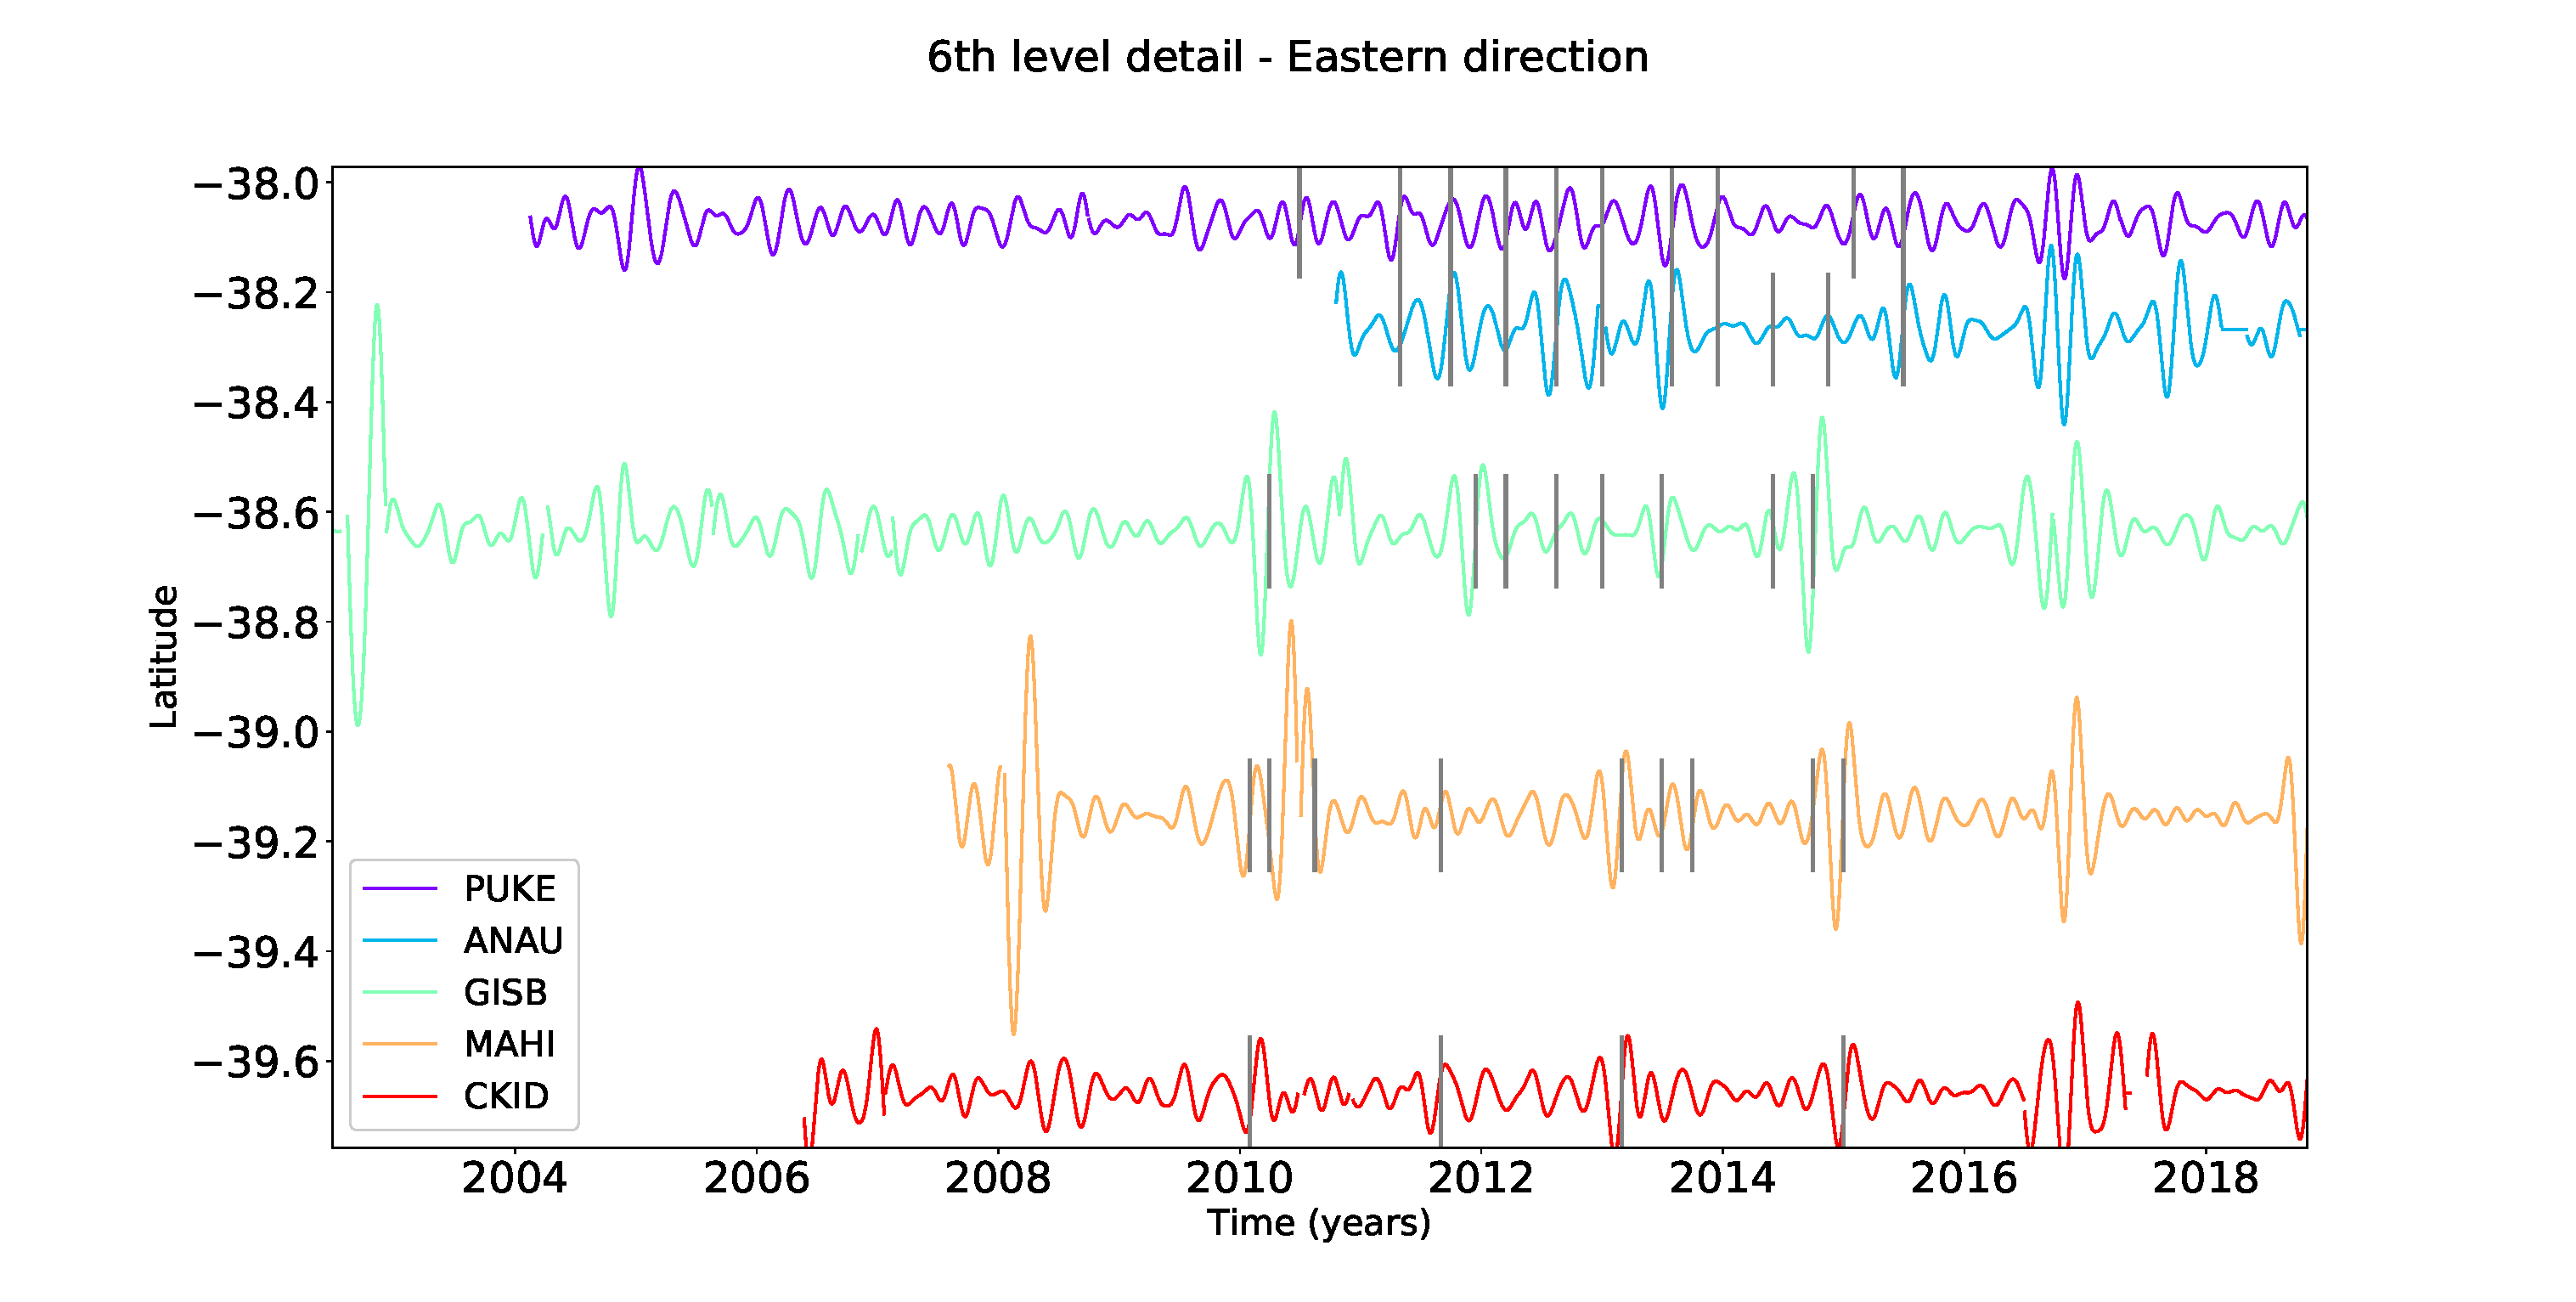
\includegraphics[trim={2.5cm 0.5cm 5cm 0.5cm}, clip, width=400pt]{figures/slowslip_MRA.eps}
\captionsetup{type=figure}
\captionof{figure}{6\textsuperscript{th} level detail of the MRA for the eastern component of the time series recorded at stations PUKE, ANAU, GISB, MAHI, and CKID. The grey bars show the time of the transients listed by Todd and Schwartz (2016 ~\cite{TOD_2016}, their Table 1).}
\end{center}

\begin{center}
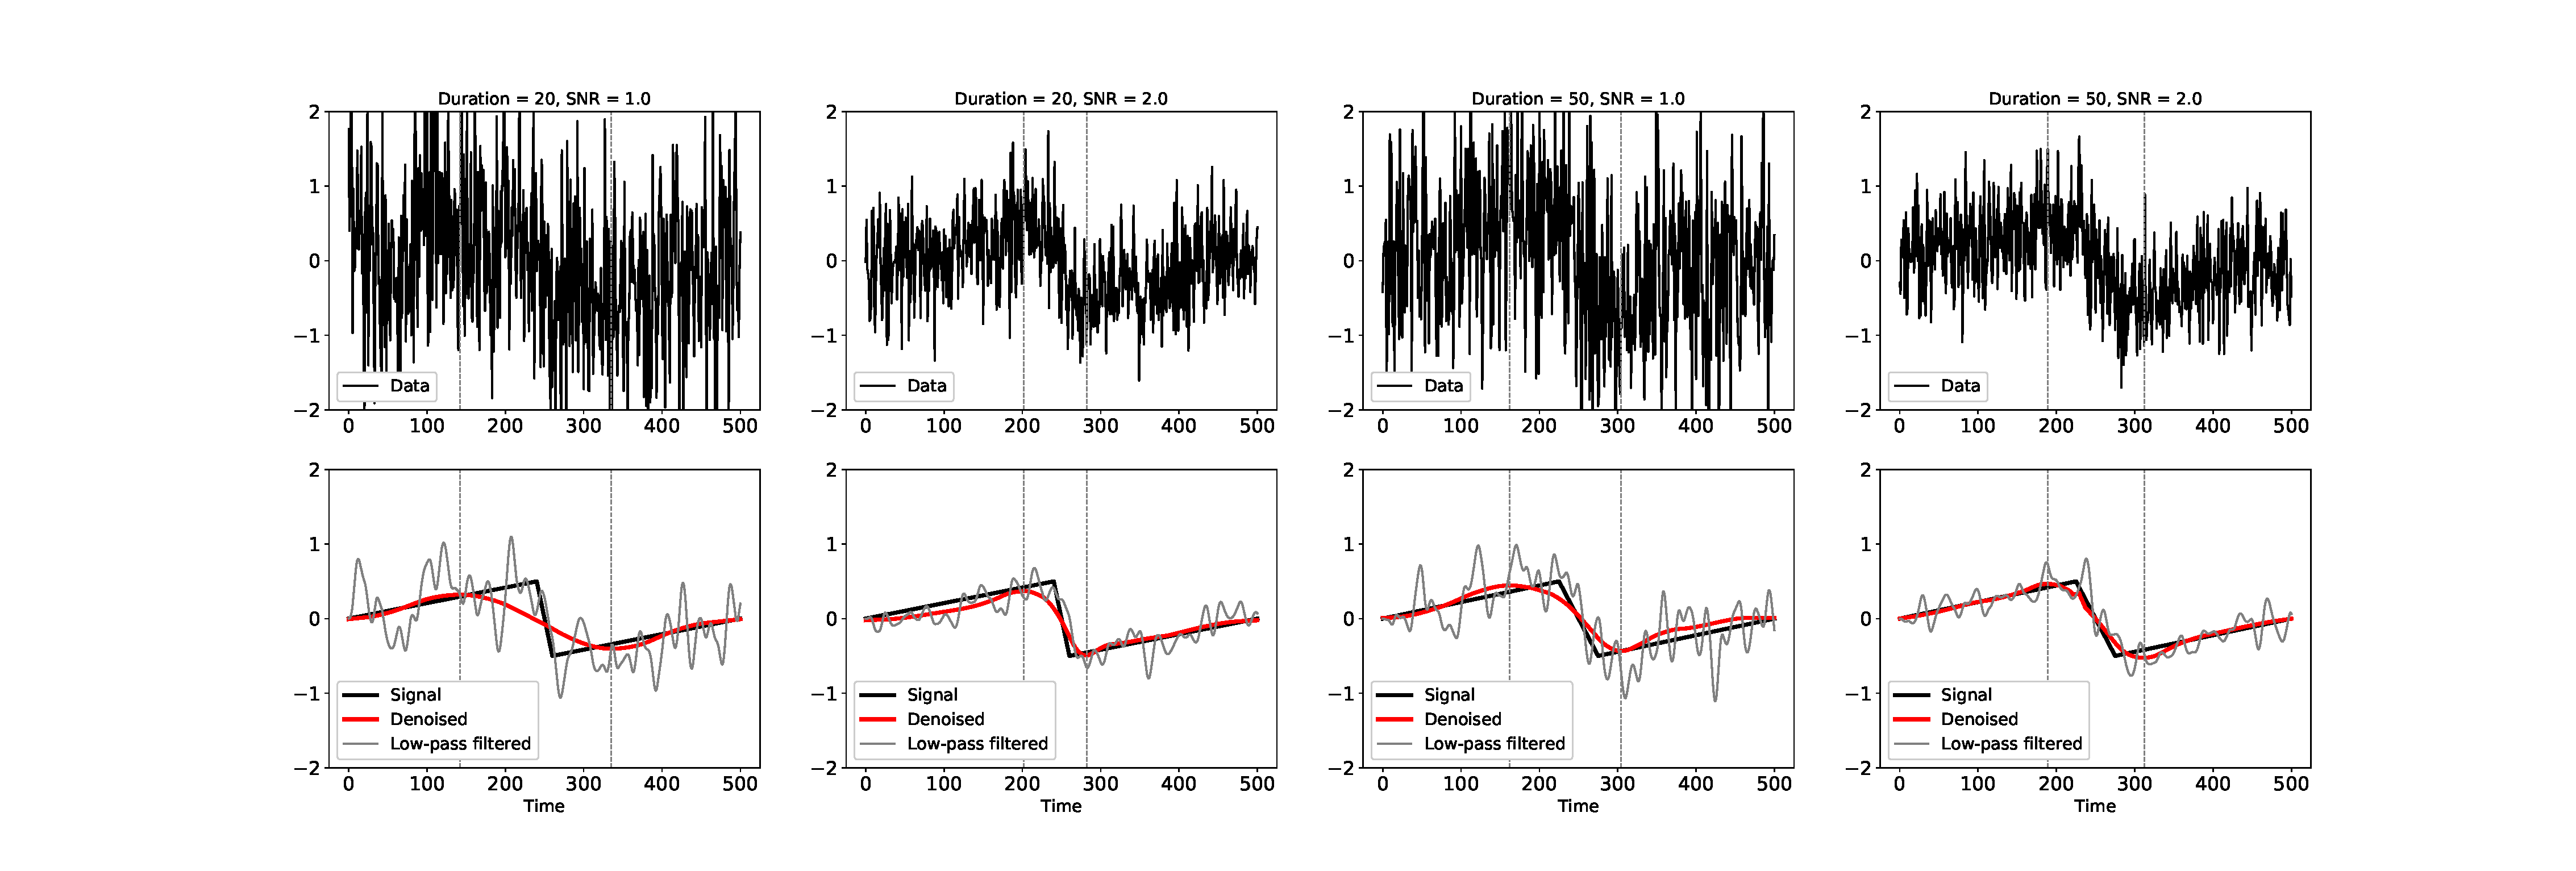
\includegraphics[trim={8.5cm 1cm 7.5cm 2cm}, clip, width=450pt]{figures/slowslip_synthetics.eps}
\captionsetup{type=figure}
\captionof{figure}{Denoising of synthetic time series using wavelets for two durations of the slow slip and two signal-to-noise ratios. The black line on the bottom panels is the signal. The black line on the top panels is the signal to which a Gaussian noise has been added. The red line on the bottom panels is the denoised signal obtained using thresholding of the wavelet vectors. The two vertical dashed lines show the time of the maxima and minima of the denoised signal. The grey line on the bottom panels is the signal obtained with a low-pass filter.}
\end{center}

\begin{center}
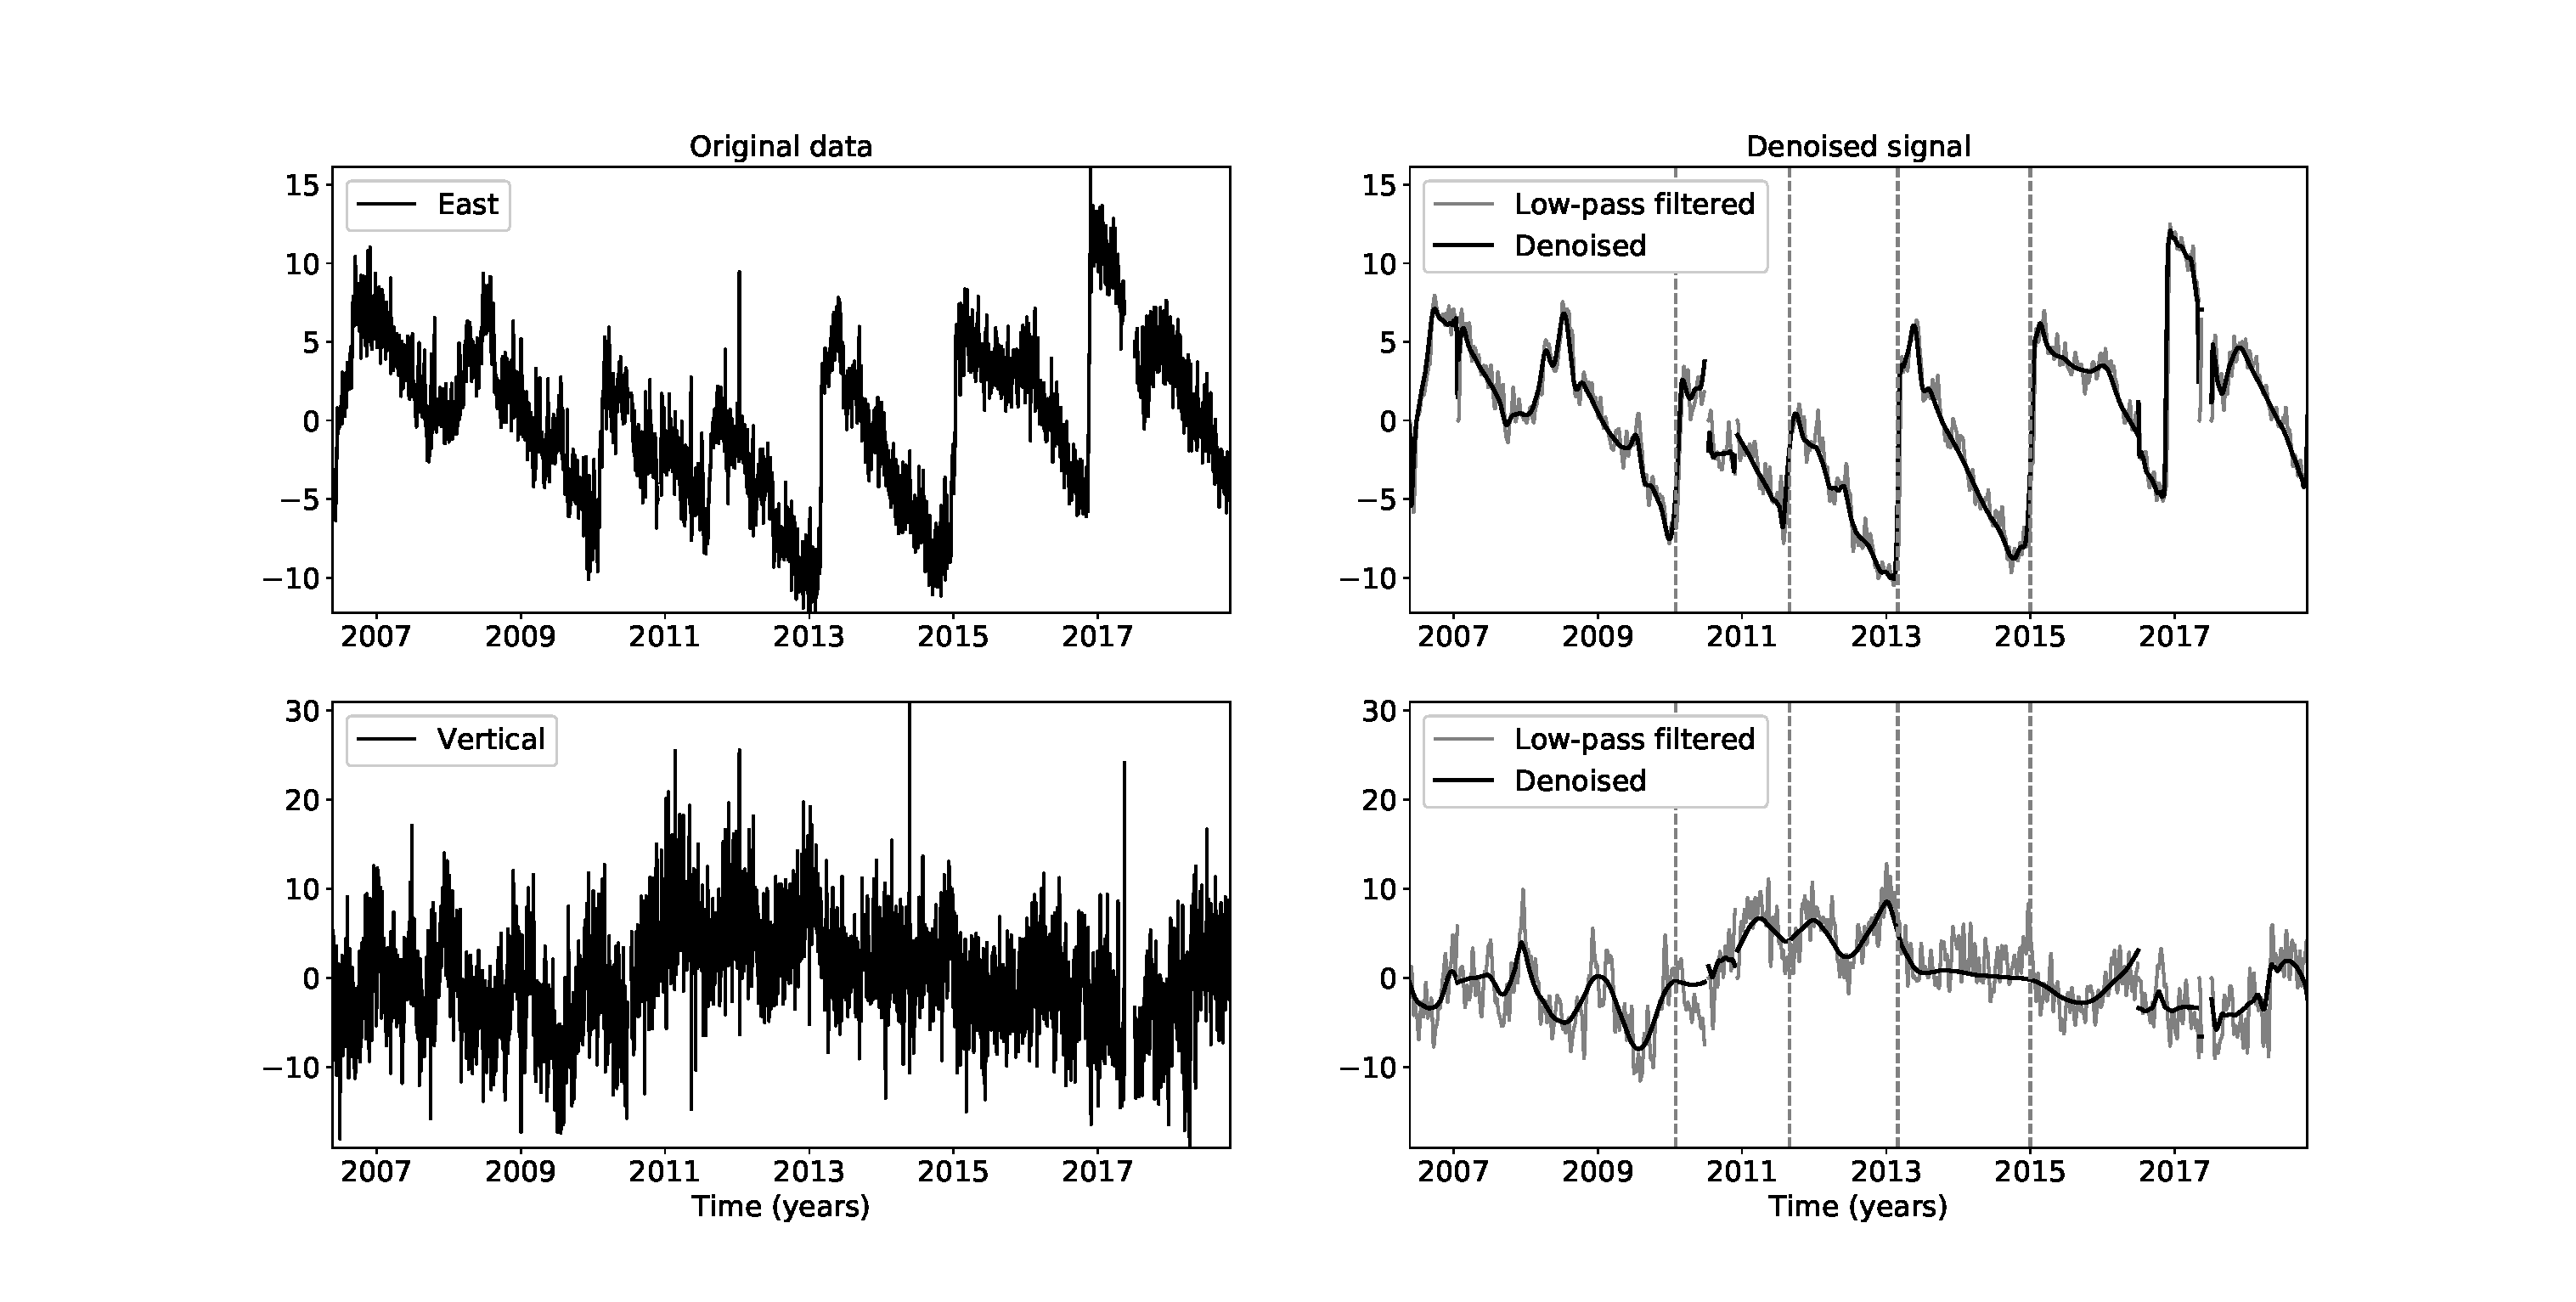
\includegraphics[trim={5cm 1cm 5cm 2cm}, clip, width=450pt]{figures/slowslip_denoising.eps}
\captionsetup{type=figure}
\captionof{figure}{Original (left) and denoised (right) displacement observed at GPS station CKID for the eastern (top) and vertical (bottom) components. The black line on the right panels is the denoised signal obtained using thresholding of the wavelet vectors. The grey line on the right panels is the signal obtained with a low-pass filter. The vertical dashed lines indicate the timing of the slow slip events identified by Todd and Schwartz (2016 ~\cite{TOD_2016}).}
\end{center}

\end{document}
